\documentclass[executivepaper]{article}

\usepackage{graphicx}
\usepackage[utf8]{inputenc}
\usepackage[T1]{fontenc}
\usepackage[spanish]{babel} % Establece el idioma español
\usepackage{csquotes} % Carga el paquete csquotes
\usepackage{graphicx} % Required for inserting images
\usepackage{listings}
\usepackage{xcolor}
\usepackage{hyperref}
\usepackage[left=1.00cm, right=1.00cm, top=2.00cm, bottom=2.00cm]{geometry}
\usepackage{tikz}
\usetikzlibrary{shapes,arrows}
\usetikzlibrary{positioning}
\setlength{\parindent}{0.5in}
\usepackage{setspace}
\doublespacing

\lstset{
    inputencoding=utf8,
    language=Java,
    basicstyle=\ttfamily,
    columns=fullflexible
}

% Define colores para el código
\definecolor{codegreen}{rgb}{0,0.6,0}
\definecolor{codegray}{rgb}{0.5,0.5,0.5}
\definecolor{codepurple}{rgb}{0.58,0,0.82}
\definecolor{backcolour}{rgb}{0.95,0.95,0.92}

% Configuración de lstlisting
\lstdefinestyle{mystyle}{
    backgroundcolor=\color{backcolour},   
    commentstyle=\color{codegreen},
    keywordstyle=\color{magenta},
    numberstyle=\tiny\color{codegray},
    stringstyle=\color{codepurple},
    basicstyle=\ttfamily\footnotesize,
    breakatwhitespace=false,         
    breaklines=true,                 
    captionpos=b,                    
    keepspaces=true,                 
    numbers=left,                    
    numbersep=5pt,                  
    showspaces=false,                
    showstringspaces=false,
    showtabs=false,                  
    tabsize=2
}

% Configuración del paquete hyperref
\hypersetup{
    colorlinks=true,
    linkcolor=black,
    filecolor=magenta,      
    urlcolor=gray,
}

\lstset{style=mystyle}

\title{Informe sobre JAVA}
\author{Kevin Cárdenas}

\begin{document}

\begin{titlepage}
    \begin{center}
        {\Huge \textbf{JAVA}}
        \\[18cm]

        \large\emph{Autor:}\\
        Kevin Cárdenas.
        \\[1cm]
        {\large 2023}
    \end{center}
\end{titlepage}

\newpage
\tableofcontents
\newpage
\section{Introducción a JAVA}
Java es un lenguaje de programación orientado a objetos diseñado para ser portable, seguro y fácil de entender. La programación orientada a objetos (POO) es una técnica de programación que se centra en la organización del código en torno a objetos, que son entidades que contienen datos y métodos para manipular esos datos.

Java es un lenguaje compilado e interpretado. Cuando se escribe un programa en Java, se escribe en un archivo fuente que luego se compila en un archivo ejecutable. Este archivo ejecutable se puede ejecutar en cualquier plataforma que tenga una máquina virtual Java (JVM) instalada. La JVM es un software que permite que los programas Java se ejecuten en diferentes sistemas operativos sin necesidad de recompilar el código fuente.

El proceso de compilación de Java convierte el código fuente en un formato binario conocido como bytecode, que es un conjunto de instrucciones que la JVM puede interpretar y ejecutar en tiempo de ejecución. La JVM interpreta el bytecode y lo convierte en código de máquina nativo para la plataforma específica en la que se está ejecutando.

En resumen, Java es un lenguaje orientado a objetos que se compila en bytecode y se interpreta en tiempo de ejecución por la JVM, lo que lo hace altamente portable y seguro.
\subsection{Instalación}
Te proporciono las instrucciones para instalar Java en Linux utilizando la terminal:
\begin{enumerate}
    \item Abre una terminal: Abre una ventana de terminal en Linux. En la mayoría de las distribuciones de Linux, puedes abrir una terminal haciendo clic en el botón de aplicaciones en la barra de tareas y buscando "terminal".
    \item Actualiza el sistema: Antes de instalar Java, asegúrate de actualizar el sistema. Para hacerlo, ejecuta el siguiente comando en la terminal:
\begin{lstlisting}[language=Bash]
sudo apt-get update    \end{lstlisting}
        Este comando actualizará la lista de paquetes disponibles en el sistema.
    \item Instala Java: Para instalar Java en Linux, puedes utilizar el comando apt-get. Ejecuta el siguiente comando en la terminal para instalar la versión más reciente de Java:
\begin{lstlisting}[language=Bash]
sudo apt-get install default-jdk\end{lstlisting}
Si deseas instalar una versión específica de Java, puedes reemplazar \enquote*{default-jdk} con el nombre de la versión que deseas instalar (por ejemplo, \enquote*{openjdk-11-jdk})
    \item Verifica la instalación: Una vez que se haya completado la instalación, verifica que Java se haya instalado correctamente. Para hacerlo, ejecuta el siguiente comando en la terminal:
\begin{lstlisting}[language=Bash]
java -version\end{lstlisting}
\end{enumerate}
Si deseas instalar inteligent IDEA sólo ejecuta el comando \lstinline{sudo snap install intellij-idea-community --classic}

Y ahora puedes escribir tu primer \enquote*{Hola Mundo}, abriendo un nuevo proyecto en nuestro IDE Creando un archivo llamado \enquote*{HolaMundo.java} y escribiendo en el lo siguiente:
\begin{lstlisting}
    public class HelloWorld {
        public static void main(String[] args) {
            System.out.println("Hola Mundo!");
        }
    }
\end{lstlisting}
    comienza con la definición de la clase "HelloWorld". Todas las clases de Java deben tener una definición como esta. La clase principal del programa debe tener el mismo nombre que el archivo de código fuente (en este caso, \enquote*{HolaMundo.java}).

    Dentro de la clase \enquote*{HelloWorld}, se define un método llamado \enquote*{main}. Este método es el punto de entrada del programa. Todos los programas de Java deben tener un método \enquote*{main} como este.

    Dentro del método \enquote*{main}, se utiliza la función \enquote*{println} de la clase \enquote*{System} para imprimir el mensaje \enquote*{Hola Mundo!} en la consola. El mensaje debe estar entre comillas dobles para indicar que es una cadena de texto.

\subsection{Tipos de Variables}

En Java, existen diferentes tipos de variables que se pueden utilizar para almacenar diferentes tipos de datos. Algunos de los tipos de variables más comunes en Java son:

\begin{itemize}
\item \textbf{int}: este tipo de variable se utiliza para almacenar valores enteros. Por ejemplo: \lstinline{int edad = 30;}
\item \textbf{double}: este tipo de variable se utiliza para almacenar valores decimales. Por ejemplo: \lstinline{double altura = 1.75;}
\item \textbf{boolean}: este tipo de variable se utiliza para almacenar valores booleanos (verdadero o falso). Por ejemplo: \lstinline{boolean esMayorDeEdad = true;}
\item \textbf{char}: este tipo de variable se utiliza para almacenar caracteres individuales. Por ejemplo: \lstinline{char inicial = 'J';}
\item \textbf{String}: este tipo de variable se utiliza para almacenar cadenas de texto. A diferencia de los otros tipos, la sintaxis de una variable de tipo String se escribe con mayúscula al inicio. Por ejemplo: \lstinline{String nombre = "Juan";}
\end{itemize}

Además de estos tipos de variables básicos, existen otros tipos más complejos en Java, como arreglos, listas, objetos, etc.

Es importante tener en cuenta que las variables en Java son de tipado estático, lo que significa que una vez que se ha declarado el tipo de una variable, no se puede cambiar. Esto ayuda a prevenir errores comunes en tiempo de ejecución.

Por ejemplo:
\begin{lstlisting}
public class EjemploVariables {

    public static void main(String[] args) {

        int edad = 30;
        double altura = 1.75;
        boolean esMayorDeEdad = true;
        char inicial = 'J';
        String nombre = "Juan";

        System.out.println("Nombre: " + nombre);
        System.out.println("Edad: " + edad);
        System.out.println("Altura: " + altura);
        System.out.println("Es mayor de edad?: " + esMayorDeEdad);
        System.out.println("Inicial: " + inicial);
    }
\end{lstlisting}

En este ejemplo, se declaran variables de diferentes tipos y se les asignan valores. Luego, se imprimen los valores de estas variables en la consola utilizando el método \enquote*{println} de la clase \enquote*{System}. La salida del programa sería la siguiente:
\begin{lstlisting}[numbers=none]
Nombre: Juan
Edad: 30
Altura: 1.75
Es mayor de edad?: true
Inicial: J
\end{lstlisting}
En este caso, el programa imprime los valores de las variables \enquote*{nombre}, \enquote*{edad}, \enquote*{altura}, \enquote*{esMayorDeEdad} e \enquote*{inicial}. Cada valor se concatena con una cadena de texto que describe qué valor se está imprimiendo.

En programación orientada a objetos (POO), además de los tipos de variables primitivos como \lstinline{int}, \lstinline{double}, \lstinline{boolean} y \lstinline{char}, existen también los tipos de variables de objeto, que se definen a partir de clases.

Los tipos de variables de objeto se utilizan para representar objetos de una clase. Por ejemplo, si tenemos una clase \lstinline{Persona}, podemos crear un objeto \lstinline{persona1} de esa clase y utilizar una variable para hacer referencia a ese objeto:

\begin{lstlisting}[language=Java]
Persona persona1 = new Persona();
\end{lstlisting}

En este caso, \lstinline{persona1} es una variable de tipo \lstinline{Persona} que hace referencia a un objeto de la clase \lstinline{Persona}. Podemos utilizar métodos y propiedades de la clase \lstinline{Persona} para interactuar con el objeto al que hace referencia la variable \lstinline{persona1}.

Además, en POO también existe el concepto de variables de instancia y variables de clase. Las variables de instancia son variables que se definen en una clase y que pertenecen a cada objeto creado a partir de esa clase. Por ejemplo, si tenemos una clase \lstinline{Persona} con una variable de instancia \lstinline{nombre}, cada objeto \lstinline{persona1}, \lstinline{persona2}, etc. tendría su propio valor de la variable \lstinline{nombre}.

Por otro lado, las variables de clase se definen en una clase y son compartidas por todos los objetos creados a partir de esa clase. Para definir una variable de clase, se utiliza la palabra clave \lstinline{static}. Por ejemplo, si queremos tener una variable \lstinline{contador} que cuente la cantidad de objetos \lstinline{Persona} creados, podemos definirla como una variable de clase:

\begin{lstlisting}[language=Java]
public class Persona {
    static int contador = 0;
    String nombre;
    public Persona(String nombre) {
        this.nombre = nombre;
        contador++;
    }
}
\end{lstlisting}

En este caso, la variable \lstinline{contador} se incrementa cada vez que se crea un objeto \lstinline{Persona}. Todas las instancias de la clase \lstinline{Persona} comparten la misma variable \lstinline{contador}.

\subsubsection*{Longitud de un número}
El tipo de dato \enquote*{int} en Java es un tipo primitivo que representa números enteros. Este tipo de dato es utilizado para almacenar valores numéricos que no tienen decimales, y ocupa 32 bits (4 bytes) en la memoria.

Esto significa que un valor de tipo \enquote*{int} puede representar cualquier número entero en el rango de \enquote*{-2,147,483,648} a \enquote*{2,147,483,647}. Si intentamos almacenar un valor fuera de este rango, se producirá un error en tiempo de ejecución.

Es importante tener en cuenta que el tipo de dato \enquote*{int} es de tamaño fijo, lo que significa que siempre ocupa la misma cantidad de memoria, independientemente del valor que esté almacenando. Esto lo hace más eficiente en términos de memoria que otros tipos de datos que permiten una mayor precisión, como el tipo \enquote*{double} o \enquote*{float}.

Si necesitamos almacenar números enteros fuera del rango de un \enquote*{int}, podemos utilizar tipos de datos de mayor tamaño, como \enquote*{long}, que ocupa 64 bits (8 bytes) en la memoria y puede almacenar valores en el rango de \enquote*{-9,223,372,036,854,775,808} a \enquote*{9,223,372,036,854,775,807}.

\subsubsection*{Diferencia entre float y double}
En Java, existen dos tipos de datos de punto flotante: \textbf{float} y \textbf{double}. Ambos se utilizan para representar números decimales, pero difieren en su precisión y tamaño en memoria.

El tipo de dato \textbf{float} ocupa 32 bits en memoria y tiene una precisión de aproximadamente 6-7 dígitos decimales significativos. Por otro lado, el tipo de dato \textbf{double} ocupa 64 bits en memoria y tiene una precisión de aproximadamente 15-16 dígitos decimales significativos.

Por lo tanto, se recomienda utilizar el tipo de dato \textbf{float} cuando se necesita una precisión menor y se quiere ahorrar memoria. Por ejemplo, cuando se trabaja con grandes cantidades de datos en una aplicación. Por otro lado, se recomienda utilizar el tipo de dato \textbf{double} cuando se necesita una mayor precisión y no se tiene restricción en cuanto al uso de memoria.

Es importante tener en cuenta que al asignar valores a variables de tipo \textbf{float} o \textbf{double}, se deben incluir los sufijos \textbf{f} o \textbf{d}, respectivamente. Por ejemplo:

\begin{lstlisting}[language=Java]
float numeroFloat = 3.14159f;
double numeroDouble = 3.14159d;
\end{lstlisting}

De lo contrario, el compilador de Java asumirá que se trata de un valor de tipo \textbf{double}.

\subsubsection*{Tipo de dato char}
El tipo de dato \lstinline{char} en Java es utilizado para almacenar un único carácter alfanumérico o un símbolo en Unicode. La sintaxis para declarar una variable de tipo \lstinline{char} es la siguiente:

\begin{lstlisting}[language=Java]
char variableChar = 'a';
\end{lstlisting}

Aquí, se declara una variable llamada \lstinline{variableChar} de tipo \lstinline{char}, y se le asigna el valor de la letra 'a'. Es importante notar que los valores de tipo \lstinline{char} siempre deben estar encerrados en comillas simples.

Además, el tipo de dato \lstinline{char} también puede representar valores numéricos utilizando su representación en la tabla ASCII. Por ejemplo:

\begin{lstlisting}[language=Java]
char variableNum = 65;
\end{lstlisting}

Aquí, la variable \lstinline{variableNum} de tipo \lstinline{char} representa el valor numérico 65 en la tabla ASCII, que es la letra 'A'. Es importante mencionar que la representación en ASCII está limitada a los caracteres del conjunto ASCII, por lo que algunos caracteres especiales pueden no tener una representación ASCII válida.

Es importante tener en cuenta que una variable \lstinline{char} ocupa 2 bytes de memoria en Java. Esto significa que puede representar valores de caracteres Unicode que se encuentran en el rango de 0 a 65,535.

\subsubsection*{Tipo de dato boolean}
El tipo de dato \textbf{boolean} en Java es un tipo de dato que puede tener dos valores: \textbf{true} o \textbf{false}. Este tipo de dato es útil cuando se desea representar una condición lógica en el programa.

A diferencia de otros tipos de datos como int o double, que pueden tener una amplia gama de valores, un boolean solo puede tener dos posibles valores. Estos valores son útiles para representar situaciones donde una condición es verdadera o falsa, como por ejemplo en una sentencia de control de flujo como un \textbf{if} o un \textbf{while}.

Es importante recordar que los valores true y false en Java son sensibles a mayúsculas y minúsculas. Además, el tipo de dato boolean solo ocupa un bit en la memoria, lo que lo convierte en uno de los tipos de datos más eficientes en términos de espacio de almacenamiento.

\subsubsection*{Tipo de dato var}
A partir de Java 10, se introdujo el tipo de dato \texttt{var}, que permite al compilador inferir el tipo de la variable en tiempo de compilación.

En lugar de declarar una variable como:

\begin{lstlisting}[language=Java]
String nombre = "Juan";
\end{lstlisting}

Podemos usar \texttt{var}:

\begin{lstlisting}[language=Java]
var nombre = "Juan";
\end{lstlisting}

En este caso, el compilador inferirá que el tipo de la variable \texttt{nombre} es \texttt{String}. También podemos usar \texttt{var} para tipos de datos más complejos, como colecciones:

\begin{lstlisting}[language=Java]
var lista = new ArrayList<String>();
\end{lstlisting}

En este caso, el compilador infiere que el tipo de la variable \texttt{lista} es \texttt{ArrayList<String>}. Sin embargo, es importante tener en cuenta que el tipo de la variable no es dinámico, una vez que se ha inferido en tiempo de compilación, el tipo de la variable no puede cambiar.

El uso de \texttt{var} puede hacer que el código sea más conciso y fácil de leer, especialmente en casos donde el tipo de dato es complejo o largo de escribir. Sin embargo, también puede hacer que el código sea menos legible si se abusa de su uso o si no se usa con cuidado.

\subsubsection*{Variables constantes}
En Java, también se pueden declarar variables que no pueden cambiar su valor después de haber sido inicializadas. Estas variables se llaman \textbf{variables constantes} o \textbf{constantes} y se declaran utilizando la palabra clave \lstinline{final}.
Por convención, el nombre de las constantes se escribe en mayúsculas y se separan las palabras con guiones bajos (\lstinline{CONSTANTE_EJEMPLO}).
Por ejemplo, podemos declarar una constante para el valor de PI de la siguiente manera:

\subsubsection{Arrays en Java}

Un arreglo (\textbf{array}) en Java es una estructura de datos que permite almacenar un conjunto de elementos del mismo tipo. Los elementos de un array se almacenan en posiciones consecutivas de memoria y se acceden mediante un índice numérico.

Para declarar un array en Java, se debe especificar el tipo de datos de los elementos y la cantidad de elementos que tendrá el array. Por ejemplo, para declarar un array de enteros con 5 elementos, se utilizaría la siguiente sintaxis:

\begin{lstlisting}[language=Java]
int[] miArray = new int[5];
\end{lstlisting}

Es importante tener en cuenta que los índices en un array comienzan en cero y terminan en el tamaño del array menos uno. Por ejemplo, si se tiene un array de enteros con 5 elementos, el primer elemento se accedería con el índice 0 y el último con el índice 4.

Además de la declaración básica de un array, existen varios métodos útiles para manipularlos en Java:

\begin{itemize}
\item \textbf{length}: devuelve la longitud del array.
\item \textbf{clone}: crea una copia exacta del array.
\item \textbf{sort}: ordena los elementos del array en orden ascendente.
\end{itemize}

También es posible declarar arrays multidimensionales en Java, es decir, arrays que contienen otros arrays como elementos. Por ejemplo, se podría declarar un array bidimensional de enteros de la siguiente manera:

\begin{lstlisting}[language=Java]
int[][] miArrayBidimensional = new int[3][2];
\end{lstlisting}

Este array tendría 3 elementos, cada uno de los cuales sería un array de enteros con 2 elementos. Para acceder a un elemento específico de un array multidimensional, se deben utilizar índices separados por comas. Por ejemplo, para acceder al segundo elemento del primer array del array bidimensional anterior, se utilizaría la siguiente sintaxis:

\begin{lstlisting}[language=Java]
int segundoElemento = miArrayBidimensional[0][1];
\end{lstlisting}

Es importante tener en cuenta que los arrays en Java tienen un tamaño fijo una vez que se han creado. Si se necesita una estructura de datos dinámica que permita agregar o eliminar elementos, se recomienda utilizar las colecciones de Java, como por ejemplo ArrayList.

\subsubsection*{Índices y búsqueda de elementos en Arrays}

Los elementos de un array en Java se pueden acceder mediante su índice. El índice de un elemento en un array es un número entero que indica su posición dentro del array. En Java, los índices comienzan en cero, lo que significa que el primer elemento de un array tiene un índice de cero, el segundo elemento tiene un índice de uno, y así sucesivamente.

Para acceder a un elemento en un array, se utiliza la sintaxis de corchetes []. El índice del elemento deseado se coloca entre los corchetes. Por ejemplo, si queremos acceder al tercer elemento de un array llamado "numeros", se utiliza la siguiente sintaxis:

\begin{lstlisting}[language=Java]
int[] numeros = {1, 2, 3, 4, 5};
int tercerNumero = numeros[2]; // Tercer elemento, indice 2
\end{lstlisting}

En este ejemplo, el tercer elemento del array \enquote*{numeros} tiene un índice de 2, por lo que se utiliza la sintaxis \enquote*{numeros[2]} para acceder a ese elemento.

Para buscar un elemento en un array, se puede utilizar un ciclo \enquote*{for} para iterar a través de todos los elementos y comparar cada uno con el elemento deseado. Sin embargo, Java también proporciona un método llamado \enquote*{binarySearch()} que puede buscar un elemento en un array ordenado de manera eficiente.

El método \enquote*{binarySearch()} utiliza el algoritmo de búsqueda binaria para encontrar el elemento deseado en el array. El algoritmo de búsqueda binaria funciona dividiendo el array en dos mitades y comparando el elemento deseado con el elemento en el medio. Si el elemento deseado es menor que el elemento en el medio, se busca en la mitad inferior del array. Si es mayor, se busca en la mitad superior del array. Este proceso se repite hasta que se encuentra el elemento deseado o se determina que no está presente en el array.

El método \enquote*{binarySearch()} tiene la siguiente sintaxis:

\begin{lstlisting}[language=Java]
Arrays.binarySearch(array, elemento);
\end{lstlisting}

Donde \enquote*{array} es el array en el que se desea buscar el elemento, y \enquote*{elemento} es el elemento que se desea buscar. El método devuelve el índice del elemento si se encuentra en el array, o un número negativo que indica el punto de inserción si el elemento no está presente en el array.

Además del método \enquote*{binarySearch()}, Java proporciona otros métodos útiles para trabajar con arrays, como \enquote*{sort()}, que ordena los elementos de un array en orden ascendente, y \enquote*{equals()}, que compara dos arrays para determinar si son iguales.

\subsubsection{Uso de variables}
Para utilizar una variable en Java, primero se debe declarar, lo que significa reservar un espacio en memoria para la variable. La declaración de una variable se realiza especificando el tipo y el nombre de la variable, como se muestra en el siguiente ejemplo:

\begin{lstlisting}[language=Java]
int edad;
\end{lstlisting}
En este caso, se está declarando una variable de tipo \lstinline{int} llamada \lstinline{edad}. Después de la declaración, se puede asignar un valor a la variable utilizando el operador de asignación \lstinline{=}, como se muestra a continuación:

\begin{lstlisting}[language=Java]
edad = 25;
\end{lstlisting}
En este caso, se está asignando el valor \lstinline{25} a la variable \lstinline{edad}.

También se puede declarar y asignar un valor a una variable en la misma línea, como se muestra en el siguiente ejemplo:

\begin{lstlisting}[language=Java]
double precio = 10.99;
\end{lstlisting}
En este caso, se está declarando una variable de tipo \lstinline{double} llamada \lstinline{precio} y se le está asignando el valor \lstinline{10.99}.

Una vez que se ha declarado y asignado un valor a una variable, se puede utilizar en el código para hacer cálculos y tomar decisiones. Por ejemplo:

\begin{lstlisting}[language=Java]
int edad = 25;
if (edad >= 18) {
System.out.println("Eres mayor de edad");
} else {
System.out.println("Eres menor de edad");
}
\end{lstlisting}
En este caso, se está utilizando la variable \lstinline{edad} para determinar si una persona es mayor o menor de edad.

También se puede actualizar el valor de una variable utilizando el operador de asignación. Por ejemplo:

\begin{lstlisting}[language=Java]
int contador = 0;
contador = contador + 1;
\end{lstlisting}
En este caso, se está incrementando el valor de la variable \lstinline{contador} en uno.

Es importante tener en cuenta que las variables en Java ocupan espacio en memoria y que este espacio es limitado. Por lo tanto, es importante utilizar variables de manera eficiente e intentar no crear más variables de las necesarias. Además, las variables que ya no se necesitan podriamos eliminarlas para liberar espacio en memoria y evitar fugas de memoria.

\subsubsection{Convención de nombres}
La convención de nombres en programación es importante para escribir código legible y fácilmente comprensible. En Java, existen algunas reglas de convención de nombres que se deben seguir para escribir código legible y coherente.

Primero, es importante recordar que Java es sensible a mayúsculas y minúsculas, lo que significa que una letra mayúscula se considera diferente de su contraparte en minúscula. Por ejemplo, la variable \enquote*{nombre} es diferente de la variable \enquote*{Nombre} en Java.

Además, existen algunas convenciones de nomenclatura comunes que se utilizan en Java. Por ejemplo, las variables generalmente se nombran usando una convención llamada \enquote*{camelCase}. En camelCase, el primer carácter de la primera palabra es en minúscula, y la primera letra de cada palabra subsiguiente se escribe en mayúscula. Por ejemplo, \enquote*{nombreDeUsuario} es un buen nombre de variable en camelCase.

En cuanto a los caracteres permitidos en los nombres de variables en Java, estos pueden contener letras, números y guiones bajos. Sin embargo, el primer carácter de un nombre de variable no puede ser un número. Además, los nombres de variables no pueden incluir espacios ni caracteres especiales como signos de puntuación o símbolos matemáticos.

Es importante seguir estas convenciones de nomenclatura para que el código sea fácil de leer y entender. Además, seguir las convenciones de nomenclatura también puede ayudar a prevenir errores en el código y hacer que sea más fácil de mantener y actualizar en el futuro.

El libro \enquote*{Clean Code} de Robert C. Martin es una gran referencia para escribir código limpio y legible. Aquí hay un resumen de algunos de los conceptos clave:
\begin{itemize}
    \item Nombres descriptivos: Elige nombres que describan claramente lo que hace una variable, método o clase. Nombres descriptivos hacen que el código sea más fácil de entender y de mantener.
    \item Funciones y métodos cortos: Las funciones y los métodos deben ser lo más cortos posible, idealmente menos de 20 líneas de código. Esto hace que el código sea más fácil de entender y de probar.
    \item Mantener un estilo consistente: Es importante mantener un estilo consistente en todo el código, desde la indentación hasta la nomenclatura de las variables. Esto hace que el código sea más fácil de leer y de mantener.
    \item Eliminar duplicación: La duplicación de código puede ser un problema importante en el código, ya que hace que el código sea más difícil de mantener y actualizar. Es importante identificar y eliminar la duplicación siempre que sea posible.
    \item Comentarios: Los comentarios deben ser utilizados para explicar el por qué del código, no el qué. El código debe ser lo suficientemente claro para entender lo que está haciendo sin necesidad de comentarios. Los comentarios pueden ser útiles para explicar decisiones arquitectónicas o decisiones de diseño.
    \item Pruebas unitarias: Las pruebas unitarias son esenciales para escribir código limpio y de calidad. Las pruebas unitarias aseguran que el código funciona correctamente y que los cambios en el código no introducen nuevos errores.
    \end{itemize}
Estos son sólo algunos de los conceptos clave que se discuten en \enquote*{Clean Code}. Siguiendo estos principios, podemos escribir código limpio y fácil de entender que es más fácil de mantener y actualizar en el futuro.    

\subsubsection*{Convención de nombres: Upper Camel Case y Lower Camel Case}
En Java, se utilizan dos convenciones de nombres comunes: Upper Camel Case y Lower Camel Case.

\textbf{Upper Camel Case}, también conocido como \textbf{PascalCase}, se utiliza para nombrar clases y tipos de datos. En Upper Camel Case, la primera letra de cada palabra se escribe en mayúscula, y no se utilizan espacios ni guiones bajos para separar las palabras. Por ejemplo:

\begin{lstlisting}[language=Java]
public class MiClaseEjemplo {
// class code
}
\end{lstlisting}

\textbf{Lower Camel Case}, también conocido como \textbf{camelCase}, se utiliza para nombrar variables, métodos y funciones. En Lower Camel Case, la primera letra de la primera palabra se escribe en minúscula, y la primera letra de cada palabra siguiente se escribe en mayúscula. No se utilizan espacios ni guiones bajos para separar las palabras. Por ejemplo:

\begin{lstlisting}[language=Java]
int edadDelUsuario = 25;
public void miMetodoEjemplo() {
// method code
}
\end{lstlisting}

\subsection{Operadores}
En programación, los operadores son símbolos o palabras reservadas que se utilizan para realizar operaciones matemáticas o lógicas sobre variables o valores. En Java, existen diferentes tipos de operadores que se utilizan en distintas situaciones.

\subsubsection*{Operadores aritméticos}

Los operadores aritméticos se utilizan para realizar operaciones matemáticas básicas entre variables numéricas. Los operadores aritméticos en Java son los siguientes:

\begin{itemize}
\item Suma (+): se utiliza para sumar dos valores.
\item Resta (-): se utiliza para restar un valor de otro.
\item Multiplicación (*): se utiliza para multiplicar dos valores.
\item División (/): se utiliza para dividir un valor por otro.
\item Módulo (\%): se utiliza para obtener el resto de una división.
\end{itemize}

\subsubsection*{Operadores de asignación}

Los operadores de asignación se utilizan para asignar un valor a una variable. El operador de asignación en Java es el signo igual (=). También existen operadores de asignación compuestos, que realizan una operación y luego asignan el resultado a la variable. Algunos ejemplos son:

\begin{itemize}
\item +=: suma el valor de la variable y el valor especificado y asigna el resultado a la variable.
\item -=: resta el valor especificado de la variable y asigna el resultado a la variable.
\item *=: multiplica el valor de la variable y el valor especificado y asigna el resultado a la variable.
\item /=: divide el valor de la variable por el valor especificado y asigna el resultado a la variable.
\item \%=: obtiene el resto de la división entre la variable y el valor especificado y asigna el resultado a la variable.
\end{itemize}

\subsubsection*{Operadores de comparación}

Los operadores de comparación se utilizan para comparar dos valores y devuelven un valor booleano (verdadero o falso) como resultado. Los operadores de comparación en Java son los siguientes:

\begin{itemize}
\item Igual que (==): devuelve verdadero si los dos valores son iguales.
\item Distinto que (!=): devuelve verdadero si los dos valores son distintos.
\item Mayor que ($>$): devuelve verdadero si el primer valor es mayor que el segundo valor.
\item Menor que ($<$): devuelve verdadero si el primer valor es menor que el segundo valor.
\item Mayor o igual que ($>=$): devuelve verdadero si el primer valor es mayor o igual que el segundo valor.
\item Menor o igual que ($<=$): devuelve verdadero si el primer valor es menor o igual que el segundo valor.
\end{itemize}

\subsubsection*{Operadores lógicos}

Los operadores lógicos son aquellos que se utilizan para realizar operaciones booleanas entre dos expresiones, cuyo resultado será verdadero o falso. Los operadores lógicos en Java son los siguientes:

\begin{itemize}
\item \textbf{AND lógico (\&\&)}: Este operador devuelve verdadero si ambas expresiones son verdaderas.
\item \textbf{OR lógico ($||$)}: Este operador devuelve verdadero si al menos una de las expresiones es verdadera.
\item \textbf{NOT lógico (!)}: Este operador se utiliza para negar el resultado de una expresión booleana. Si la expresión original es verdadera, el resultado será falso, y viceversa.
\end{itemize}

A continuación, se muestran algunos ejemplos de uso de operadores lógicos:

\begin{lstlisting}[language=Java]
boolean a = true;
boolean b = false;

boolean c = a && b; // false

boolean d = a || b; // true

boolean e = !a; // false
\end{lstlisting}


Podemos hacer un ejemplo sencillo que combine varios conceptos que hemos visto. Por ejemplo, podemos escribir un programa que le pregunte al usuario su edad y, dependiendo de si es mayor o menor de edad, le dé la bienvenida o le indique que debe esperar un poco más para poder acceder al contenido.

Vamos a crear un programa que permita al usuario ingresar su edad y verifique si es mayor de edad o no. Para ello, utilizaremos los conceptos vistos anteriormente.

\begin{lstlisting}[language=Java]
import java.util.Scanner;
    
public class Main {
    public static void main(String[] args) {
    Scanner input = new Scanner(System.in);
    System.out.print("Ingrese su edad: ");
    int edad = input.nextInt();

    boolean esMayorDeEdad = edad >= 18;

    System.out.println("Usted tiene " + edad + " a~nos.");
    System.out.println("Es mayor de edad?: " + esMayorDeEdad);
}
}
\end{lstlisting}

En este programa, utilizamos la clase \lstinline{Scanner} para leer la entrada del usuario desde la consola. Luego, guardamos la edad ingresada en una variable de tipo \lstinline{int} llamada \lstinline{edad}.

Después, utilizamos una variable de tipo \lstinline{boolean} llamada \lstinline{esMayorDeEdad} para verificar si la edad ingresada es mayor o igual a 18 años.

Finalmente, imprimimos la edad ingresada y si el usuario es mayor de edad o no utilizando la función \lstinline{println} de la clase \lstinline{System} y concatenando las variables correspondientes.

\subsubsection{Operaciones matemáticas con Math}
En Java, la clase Math proporciona una serie de métodos estáticos para realizar operaciones matemáticas. A continuación se muestran algunos ejemplos:

\begin{itemize}
    \item \enquote*{\textbf{max}}: El método \enquote*{max} de Math toma dos números como argumentos y devuelve el mayor de los dos. Por ejemplo:
    \begin{lstlisting}[language=Java]
    int a = 10;
    int b = 20;
    int maximo = Math.max(a, b); // devuelve 20
    \end{lstlisting}
    \item \enquote*{\textbf{min}}: El método \enquote*{min} de Math toma dos números como argumentos y devuelve el menor de los dos. Por ejemplo:
\begin{lstlisting}[language=Java]
int a = 10;
int b = 20;
int minimo = Math.min(a, b); // devuelve 10
\end{lstlisting}

\item \enquote*{\textbf{abs}}: El método \enquote*{abs} de Math devuelve el valor absoluto de un número. Por ejemplo:
\begin{lstlisting}[language=Java]
int a = -10;
int valorAbsoluto = Math.abs(a); // devuelve 10
\end{lstlisting}

\item \enquote*{\textbf{sqrt}}: El método \enquote*{sqrt} de Math devuelve la raíz cuadrada de un número. Por ejemplo:
\begin{lstlisting}[language=Java]
int a = 25;
double raizCuadrada = Math.sqrt(a); // devuelve 5.0
\end{lstlisting}

\item \enquote*{\textbf{pow}}: El método \enquote*{pow} de Math toma dos números como argumentos y devuelve el resultado de elevar el primer número a la potencia del segundo número. Por ejemplo:
\begin{lstlisting}[language=Java]
int base = 2;
int exponente = 3;
double potencia = Math.pow(base, exponente); // devuelve 8.0
\end{lstlisting}

\item \enquote*{\textbf{sin, cos, tan}}: Los métodos \enquote*{sin}, \enquote*{cos} y \enquote*{tan} de Math calculan el seno, coseno y tangente de un ángulo en radianes, respectivamente. Por ejemplo:
\begin{lstlisting}[language=Java]
double angulo = Math.PI / 4; // angulo de 45 grados en radianes
double seno = Math.sin(angulo); // devuelve 0.7071067811865475
double coseno = Math.cos(angulo); // devuelve 0.7071067811865476
double tangente = Math.tan(angulo); // devuelve 0.9999999999999999
\end{lstlisting}

\end{itemize}
Es importante tener en cuenta que los métodos trigonométricos de Math toman como argumento un ángulo en radianes, no en grados. Para convertir de grados a radianes, se puede utilizar la siguiente  fórmula:

$$\theta_{rad} = \frac{\theta_{grados} \times \pi}{180}$$

donde $\theta_{rad}$ es el ángulo en radianes y $\theta_{grados}$ es el ángulo en grados.

Por ejemplo, si se quisiera calcular el seno de 45 grados utilizando el método sin() de Math, se debería convertir primero a radianes utilizando la fórmula anterior:

$$45_{grados} = \frac{\pi}{4}_{radianes}$$

Entonces, el código para calcular el seno de 45 grados utilizando el método sin() sería el siguiente:

\begin{lstlisting}[language=Java]
double anguloEnGrados = 45;
double anguloEnRadianes = anguloEnGrados * Math.PI / 180;
double seno = Math.sin(anguloEnRadianes);
System.out.println("El seno de " + anguloEnGrados + " grados es: " + seno);
\end{lstlisting}
El resultado sería: \lstinline{El seno de 45.0 grados es: 0.7071067811865475}

\subsection{Casting en Variables}

El casting en Java es la conversión explícita de una variable de un tipo de dato a otro. Esto se hace poniendo entre paréntesis el tipo de dato al que se desea convertir la variable, seguido del nombre de la variable.

\subsubsection{Casting Manual}

En Java, algunos tipos de datos se pueden convertir manualmente en otros tipos de datos. Un ejemplo común es la conversión de un \texttt{double} a un \texttt{int}. Para hacer esto, simplemente se escribe el tipo de dato al que se desea convertir la variable entre paréntesis, seguido del nombre de la variable:

\begin{lstlisting}[language=Java]
double d = 10.5;
int i = (int) d;
System.out.println(i); // salida: 10
\end{lstlisting}

También se puede hacer lo contrario, es decir, convertir un \texttt{int} a un \texttt{double}:

\begin{lstlisting}[language=Java]
int i = 10;
double d = (double) i;
System.out.println(d); // salida: 10.0
\end{lstlisting}

\subsubsection{Casting Automático}

En algunos casos, Java realiza la conversión de un tipo de dato a otro de forma automática. Esto se conoce como casting automático y sucede cuando se asigna una variable de un tipo de dato a una variable de otro tipo de dato compatible. Por ejemplo, cuando se asigna una variable \texttt{int} a una variable \texttt{double}, Java convierte automáticamente el \texttt{int} a un \texttt{double}:

\begin{lstlisting}[language=Java]
int i = 10;
double d = i;
System.out.println(d); // salida: 10.0
\end{lstlisting}

Sin embargo, no todos los tipos de datos son compatibles entre sí. En estos casos, es necesario hacer un casting manual para convertir la variable.

\subsubsection{Casting en otros tipos de datos}

El casting manual también se puede utilizar en otros tipos de datos, como en el caso de los tipos de datos \texttt{char} y \texttt{boolean}. Por ejemplo, para convertir un \texttt{char} a un \texttt{int}, se puede hacer lo siguiente:

\begin{lstlisting}[language=Java]
char c = 'a';
int i = (int) c;
System.out.println(i); // salida: 97
\end{lstlisting}

Y para convertir un \texttt{boolean} a un \texttt{int}, se puede hacer lo siguiente:

\begin{lstlisting}[language=Java]
boolean b = true;
int i = b ? 1 : 0;
System.out.println(i); // salida: 1
\end{lstlisting}

Es importante tener en cuenta que los tipos de datos deben ser compatibles entre sí para poder hacer un casting automático. En caso contrario, es necesario hacer un casting manual para convertir la variable al tipo de dato deseado.

\subsection*{Versiones de Java y JDK}

Java es un lenguaje de programación popular utilizado en una variedad de aplicaciones, desde aplicaciones web hasta aplicaciones móviles. A lo largo de los años, ha habido varias versiones de Java, cada una con sus propias características y mejoras.

El Java Development Kit (JDK) es un kit de herramientas de desarrollo para Java que incluye el compilador Java, la biblioteca de clases Java y otras herramientas de desarrollo. El JDK es necesario para desarrollar y ejecutar programas en Java.

A continuación, se muestran algunas de las versiones de Java y JDK más populares:

\subsubsection*{Java SE 8}

Java SE 8 es una de las versiones más populares de Java. Fue lanzada en marzo de 2014 y es conocida por sus mejoras en el rendimiento y la seguridad. Java SE 8 también introdujo la programación funcional en Java con la adición de las expresiones lambda.

\subsubsection*{Java SE 11}

Java SE 11 es otra versión popular de Java. Fue lanzada en septiembre de 2018 y es conocida por sus mejoras en la seguridad y la estabilidad. Java SE 11 también introdujo la noción de lanzamientos a largo plazo (LTS), que son lanzamientos que reciben soporte a largo plazo.

\subsubsection*{Java SE 16}

Java SE 16 es la versión más reciente de Java en el momento de escribir esto. Fue lanzada en marzo de 2021 y es conocida por sus mejoras en la programación funcional y en la seguridad.

Es importante tener en cuenta que las diferentes versiones de Java pueden tener diferentes funcionalidades y características. Al seleccionar una versión de Java, es importante considerar las necesidades del proyecto y las características específicas de cada versión.

Además, es importante tener en cuenta que la elección del JDK también es importante para el desarrollo de programas en Java. Es recomendable utilizar la última versión del JDK para aprovechar al máximo las características y mejoras de Java.

\subsubsection*{Archivos .jar}

Un archivo JAR (Java ARchive) es un archivo comprimido que contiene código y recursos que puede ser utilizado por una máquina virtual de Java. Estos archivos suelen utilizarse para distribuir bibliotecas de clases reutilizables o aplicaciones completas escritas en Java.

Para crear un archivo .jar desde la línea de comandos, se utiliza el comando \texttt{jar} proporcionado por el JDK de Java. La sintaxis básica del comando es la siguiente:

\begin{lstlisting}[language=Java]
jar cf jar-file input-file(s)
\end{lstlisting}

Donde \texttt{jar-file} es el nombre del archivo .jar que se desea crear, y \texttt{input-file(s)} es la lista de archivos que se desean incluir en el archivo .jar. Por ejemplo, para crear un archivo .jar que contenga todos los archivos .class en el directorio actual, se puede utilizar el siguiente comando:

\begin{lstlisting}[language=Java]
jar cf mylibrary.jar *.class
\end{lstlisting}

Para utilizar una biblioteca JAR en un proyecto de Java, primero se debe agregar la biblioteca al classpath del proyecto. Esto se puede hacer de varias formas, dependiendo del entorno de desarrollo utilizado. En Eclipse, por ejemplo, se puede agregar una biblioteca JAR al classpath de un proyecto haciendo clic derecho en el proyecto, seleccionando \enquote*{Propiedades}, y luego seleccionando \enquote*{Java Build Path} en el menú de la izquierda. A continuación, se debe hacer clic en la pestaña \enquote*{Librerías}, y luego en el botón \enquote*{Agregar JARs...} para seleccionar el archivo .jar que se desea agregar.

Una vez que se ha agregado la biblioteca al classpath del proyecto, se pueden importar las clases y utilizarlas en el código de la misma manera que se importan y utilizan las clases de la biblioteca estándar de Java.

Es importante tener en cuenta que los archivos JAR pueden contener código malicioso o peligroso. Por esta razón, se debe tener precaución al descargar y utilizar archivos JAR de fuentes desconocidas.

\subsection{Ciclos en Java}

Los ciclos son estructuras de control que permiten repetir una o varias instrucciones mientras se cumpla una condición. En Java, existen varios tipos de ciclos, cada uno con su propia sintaxis y uso específico.

\subsubsection{Ciclo condicional: \texttt{if}}

El ciclo condicional \texttt{if} permite ejecutar una o varias instrucciones si se cumple una condición determinada. Su sintaxis es la siguiente:

\begin{lstlisting}[language=Java]
if (condicion) {
// Instrucciones a ejecutar si se cumple la condicion
}
\end{lstlisting}
Si la condición es verdadera, se ejecutan las instrucciones dentro del bloque de código entre llaves. Si la condición es falsa, se omite la ejecución de las instrucciones y se continúa con la siguiente línea de código. También se puede utilizar la instrucción \texttt{else} para especificar un bloque de código a ejecutar en caso de que la condición sea falsa:

\begin{lstlisting}[language=Java]
if (condicion) {
// Instrucciones a ejecutar si se cumple la condicion
} else {
// Instrucciones a ejecutar si NO se cumple la condicion
}
\end{lstlisting}

\subsubsection{\texttt{Switch} en Java}

En Java, el \texttt{switch} es una estructura de control que permite realizar diferentes acciones según el valor de una expresión. La sintaxis básica del \texttt{switch} es la siguiente:

\begin{lstlisting}[language=Java]
switch (expresion) {
    case valor1:
        // codigo para valor1
        break;
    case valor2:
        // codigo para valor2
        break;
    case valor3:
        // codigo para valor3
        break;
    default:
        // codigo para cualquier otro valor
}
\end{lstlisting}

En este ejemplo, la variable \texttt{expresion} es evaluada y se compara con cada uno de los valores especificados en los casos (\texttt{valor1}, \texttt{valor2} y \texttt{valor3}). Si el valor coincide con alguno de los casos, se ejecuta el código correspondiente a ese caso. Si no coincide con ninguno de los casos, se ejecuta el código dentro del bloque \texttt{default}.

A continuación se presenta un ejemplo práctico de cómo utilizar el \texttt{switch} en Java para calcular el día de la semana a partir de un número del 1 al 7:

\begin{lstlisting}[language=Java]
public class DiaDeLaSemana {
    public static void main(String[] args) {
        int numDia = 3;
        String dia = "";

        switch (numDia) {
            case 1:
                dia = "Lunes";
                break;
            case 2:
                dia = "Martes";
                break;
            case 3:
                dia = "Miercoles";
                break;
            case 4:
                dia = "Jueves";
                break;
            case 5:
                dia = "Viernes";
                break;
            case 6:
                dia = "Sabado";
                break;
            case 7:
                dia = "Domingo";
                break;
            default:
                dia = "Numero invalido";
        }

        System.out.println("El dia correspondiente al numero " + numDia + " es " + dia + ".");
    }
}
\end{lstlisting}

En este ejemplo, se utiliza el \texttt{switch} para asignar un valor a la variable \texttt{dia} según el valor de la variable \texttt{numDia}. Luego, se muestra por pantalla el día correspondiente al número ingresado. Si se ingresa un número que no está dentro del rango del 1 al 7, se muestra un mensaje indicando que el número es inválido.

\subsubsection{Ciclo repetitivo: \texttt{for}}

El ciclo for en Java es una estructura de control utilizada para repetir un bloque de código varias veces, mientras se cumpla una condición. En Java, existen dos tipos de ciclo for: el ciclo for normal y el ciclo for each.

\subsubsection*{Ciclo For Each}

El ciclo for each, también conocido como for mejorado, es una forma simplificada de recorrer los elementos de una colección o un arreglo en Java. En lugar de utilizar un índice para acceder a cada elemento, el ciclo for each utiliza una variable para hacer referencia a cada uno de los elementos de la colección.

La sintaxis del ciclo for each en Java es la siguiente:

\begin{lstlisting}[language=Java]
for (tipoDeDato variable : coleccion) {
// Codigo a ejecutar
}
\end{lstlisting}
En esta sintaxis, \enquote*{tipoDeDato} es el tipo de dato de la colección, \enquote*{variable} es la variable que se utilizará para hacer referencia a cada elemento de la colección y \enquote*{coleccion} es la colección que se va a recorrer.

Por ejemplo, si tenemos un arreglo de números enteros y queremos imprimir cada uno de sus elementos, podemos utilizar un ciclo for each de la siguiente manera:

\begin{lstlisting}[language=Java]
int[] numeros = {1, 2, 3, 4, 5};
for (int numero : numeros) {
System.out.println(numero);
}
\end{lstlisting}
Este código imprimirá los números 1, 2, 3, 4 y 5 en la consola.

\subsubsection*{Notación más compacta}

En Java, existen algunas formas de hacer la sintaxis del ciclo for más compacta. Por ejemplo, si queremos recorrer un arreglo desde la posición 0 hasta la posición n-1, podemos utilizar la siguiente sintaxis:

\begin{lstlisting}[language=Java]
for (int i = 0; i < n; i++) {
// Codigo a ejecutar
}
\end{lstlisting}
En esta sintaxis, \enquote*{i} es el índice del arreglo y \enquote*{n} es el tamaño del arreglo.

También es posible utilizar la notación \enquote*{++i} en lugar de \enquote*{i++} para incrementar el valor de la variable \enquote*{i} en una unidad antes de que se ejecute el bloque de código. Por ejemplo:

\begin{lstlisting}[language=Java]
for (int i = 0; i < n; ++i) {
// Codigo a ejecutar
}
\end{lstlisting}
Esta notación puede ser útil en algunos casos en los que se desea incrementar el valor de la variable antes de utilizarla en el bloque de código.

La \texttt{inicializacion} define una variable de control y su valor inicial. La \texttt{condicion} define la condición que debe cumplirse para continuar ejecutando el ciclo. El \texttt{incremento} se ejecuta después de cada iteración y permite modificar el valor de la variable de control. Si la condición es verdadera, se ejecutan las instrucciones dentro del bloque de código entre llaves. Después de cada iteración, se evalúa la condición nuevamente. Si la condición es falsa, se sale del ciclo.

\subsubsection{Ciclo repetitivo: \texttt{while}}

El ciclo repetitivo \texttt{while} permite ejecutar una o varias instrucciones mientras se cumpla una condición determinada. Su sintaxis es la siguiente:

\begin{lstlisting}[language=Java]
while (condicion) {
// Instrucciones a ejecutar mientras se cumpla la condicion
}
\end{lstlisting}

Si la condición es verdadera, se ejecutan las instrucciones dentro del bloque de código entre llaves. Después de cada ejecución, se evalúa la condición nuevamente. Si la condición es falsa, se sale del ciclo.

\subsubsection{Ciclo repetitivo: \texttt{do-while}}

El ciclo repetitivo \texttt{do-while} es similar al ciclo \texttt{while}, pero la evaluación de la condición se realiza después de la primera ejecución del bloque de código. Su sintaxis es la siguiente:

\begin{lstlisting}[language=Java]
do {
// bloque de codigo
} while (condicion);
\end{lstlisting}
    
    En este caso, el bloque de código se ejecuta al menos una vez, independientemente de si la condición es verdadera o falsa en la primera evaluación. Después de la primera ejecución, la condición se evalúa nuevamente. Si es verdadera, el bloque de código se ejecuta de nuevo y así sucesivamente, hasta que la condición se vuelva falsa.

\subsubsection{El comando \texttt{break}}

    En ocasiones, puede ser necesario detener un ciclo antes de que este termine su ejecución normal. Para esto, se utiliza el comando \texttt{break}.
    
    El comando \texttt{break} permite salir de un ciclo de manera inmediata, incluso si la condición de finalización no se ha cumplido. Su sintaxis es la siguiente:
    
    \begin{lstlisting}[language=Java]
    while (condicion) {
      // cuerpo del ciclo
      if (condicionDeSalida) {
        break;
      }
    }
    \end{lstlisting}
    
    En este ejemplo, el ciclo \texttt{while} se ejecutará mientras la condición sea verdadera. Si se cumple la condición de salida, se ejecutará el comando \texttt{break}, que hará que el ciclo se detenga inmediatamente y se salga de él.
    
    Es importante tener en cuenta que el comando \texttt{break} solo detiene el ciclo más interno en el que se encuentra. Si se están utilizando ciclos anidados, se puede utilizar el comando \texttt{break} para salir de uno de los ciclos, pero no de todos.
    
    Es posible que en algunos casos sea necesario utilizar el comando \texttt{break} en conjunto con una estructura condicional, como se muestra en el siguiente ejemplo:
    
    \begin{lstlisting}[language=Java]
    while (condicion) {
      // cuerpo del ciclo
      if (condicionDeSalida) {
        if (otraCondicion) {
          break;
        } else {
          // hacer algo
        }
      }
    }
    \end{lstlisting}
    
    En este caso, si se cumple la condición de salida, se evalúa la otra condición. Si esta es verdadera, se ejecuta el comando \texttt{break}, lo que hace que se salga del ciclo \texttt{while}. Si la otra condición es falsa, se continúa con la ejecución normal del ciclo.
    
    El uso adecuado del comando \texttt{break} puede ser de gran utilidad en situaciones en las que se necesite salir de un ciclo de manera inmediata. Sin embargo, es importante utilizarlo con cuidado, ya que su uso excesivo puede llevar a un código difícil de entender y mantener.
    

\subsubsection{Ejemplos practicos}
Te dejo un ejemplo de método de análisis numérico de bisección implementado en Java:
\begin{lstlisting}[language=Java]
public class BisectionMethod {

    public static double findRoot(double a, double b, double epsilon) {
        double mid = (a + b) / 2.0;
        while (Math.abs(a - b) > epsilon) {
            if (function(mid) == 0) {
                return mid;
            }
            if (function(a) * function(mid) < 0) {
                b = mid;
            } else {
                a = mid;
            }
            mid = (a + b) / 2.0;
        }
        return mid;
    }

    public static double function(double x) {
        // Define la funcion cuya raiz se quiere encontrar
        return Math.pow(x,2)-2;
    }

    public static void main(String[] args) {
        double a = 0;
        double b = 2;
        double epsilon = 0.001;
        double root = findRoot(a, b, epsilon);
        System.out.println("La raiz de la funcion es: " + root);
    }
}
\end{lstlisting}
Este programa calcula la raíz cuadrada de 2 usando el método de bisección. La función \texttt{f} define la función que se va a evaluar, en este caso $f(x) = x^2 - 2$. El método \texttt{bisection} toma como entrada los límites del intervalo, una tolerancia y el número máximo de iteraciones, y devuelve la aproximación de la raíz. El programa principal simplemente llama al método \texttt{bisection} con los parámetros deseados y muestra el resultado.

\subsection{Funciones}
En Java, una función se define utilizando la siguiente estructura:

\begin{lstlisting}[language=Java]
[modificadorAcceso] tipoRetorno nombreFuncion (tipoParametro1 nombreParametro1, tipoParametro2 nombreParametro2, ...) {
// Codigo de la funcion
return valorRetorno;
}
\end{lstlisting}

Donde:

\begin{itemize}
\item \textbf{modificadorAcceso} indica el nivel de acceso a la función, puede ser \texttt{public}, \texttt{private} o \texttt{protected}.
\item \textbf{tipoRetorno} es el tipo de dato que devuelve la función, puede ser un tipo primitivo o una clase.
\item \textbf{nombreFuncion} es el nombre de la función.
\item \textbf{tipoParametro} es el tipo de dato del parámetro que recibe la función.
\item \textbf{nombreParametro} es el nombre del parámetro que recibe la función.
\item \textbf{valorRetorno} es el valor que devuelve la función, debe ser del tipo de dato indicado en \texttt{tipoRetorno}.
\end{itemize}

A continuación, se muestra un ejemplo de cómo se define una función en Java:

\begin{lstlisting}[language=Java]
public int suma(int num1, int num2) {
int resultado = num1 + num2;
return resultado;
}
\end{lstlisting}

Esta función recibe dos parámetros de tipo \texttt{int} y devuelve un valor de tipo \texttt{int} que es la suma de los dos parámetros.

Es importante destacar que una función puede no tener parámetros y también puede no devolver ningún valor. En este caso, se utiliza el tipo de dato \texttt{void} para indicar que no se devuelve ningún valor. Por ejemplo:

\begin{lstlisting}[language=Java]
public void imprimirHola() {
System.out.println("Hola!");
}
\end{lstlisting}

Esta función no recibe ningún parámetro y no devuelve ningún valor, simplemente imprime en pantalla el mensaje "Hola!".


\subsubsection{Modificadores de acceso}
Los modificadores de acceso en Java se utilizan para controlar el nivel de acceso a las clases, métodos y variables. 
Los cuatro modificadores de acceso que se pueden utilizar en Java son:

\begin{itemize}
\item \texttt{public}: Los miembros públicos se pueden acceder desde cualquier parte del código. Se pueden acceder desde la propia clase, desde cualquier otra clase en el mismo paquete, desde cualquier subclase y desde cualquier clase en otro paquete.
\item \texttt{protected}: Los miembros protegidos se pueden acceder desde la propia clase, desde cualquier otra clase en el mismo paquete y desde cualquier subclase, pero no se pueden acceder desde una clase en otro paquete a menos que la clase en el otro paquete sea una subclase.
\item \texttt{default}: Los miembros con acceso predeterminado (sin especificar ningún modificador) se pueden acceder desde la propia clase y desde cualquier otra clase en el mismo paquete, pero no se pueden acceder desde cualquier subclase o desde una clase en otro paquete.
\item \texttt{private}: Los miembros privados solo se pueden acceder desde la propia clase. No se pueden acceder desde cualquier otra clase, ni siquiera de una subclase.
\end{itemize}

\subsubsection{El alcance o Scope de variables}
El alcance o scope de una variable se refiere a la parte del programa en la que se puede acceder a esa variable. Hay tres tipos de alcances de variables en Java:
\begin{itemize}
    \item \texttt{Alcance de clase}: una variable de clase tiene un alcance que es toda la clase en la que se declara. Esto significa que la variable se puede acceder desde cualquier método en la clase y desde cualquier instancia de la clase.
    \item \texttt{Alcance de instancia}: una variable de instancia tiene un alcance que es la instancia de la clase en la que se declara. Esto significa que la variable se puede acceder desde cualquier método en la instancia de la clase, pero no desde otros objetos o instancias.
    \item \texttt{Alcance local}: una variable local tiene un alcance que es el bloque de código en el que se declara. Esto significa que la variable se puede acceder solo dentro del bloque de código en el que se declara, y no desde otros bloques de código o métodos.
\end{itemize}
Aquí hay algunos ejemplos de variables en diferentes alcances en Java:
\begin{lstlisting}[language=Java]
public class ScopeExample {
// Alcance de clase
    static int variableDeClase = 1;
// Alcance de instancia
    int variableDeInstancia = 2;
    public void ejemploDeScope() {
// Alcance local
        int variableLocal = 3;
    System.out.println("Variable de clase: " + variableDeClase);
    System.out.println("Variable de instancia: " + variableDeInstancia);
    System.out.println("Variable local: " + variableLocal);
    }
}
\end{lstlisting}
En el ejemplo anterior, la variable \texttt{variableDeClase} tiene un alcance de clase, lo que significa que se puede acceder desde cualquier parte del programa que tenga acceso a la clase \texttt{ScopeExample}. La variable \texttt{variableDeInstancia} tiene un alcance de instancia, lo que significa que es accesible para todos los métodos dentro de la clase y puede ser utilizadas por cualquier objeto de esta clase. La variable \texttt{variableLoacal} tiene un alcance local, lo que significa que solo es accesiblet dentro de este método o bloque.

El alcance de una variable se puede limitar utilizando el modificador de acceso.  Las variables públicas son accesibles desde cualquier parte del código, mientras que las variables protegidas solo son accesibles por la propia clase, las subclases y otras clases dentro del mismo paquete. Las variables privadas solo son accesibles por la propia clase y no pueden ser accedidas desde ninguna otra clase. Las variables sin modificador solo son accesibles dentro del mismo paquete.



\subsection{Documentación con Javadoc}
La documentación es una parte esencial de cualquier proyecto de programación, ya que permite a otros programadores entender el propósito, funcionamiento y uso del código. En Java, una herramienta muy útil para generar documentación es Javadoc.\\

Javadoc es una herramienta que genera documentación en formato HTML a partir del código fuente y los comentarios del desarrollador. Los comentarios de Javadoc comienzan con el símbolo \texttt{/**} y terminan con el símbolo \texttt{*/}. El contenido de los comentarios de Javadoc se puede utilizar para generar documentación, incluyendo información sobre la clase, los campos, los métodos y los parámetros.\\

La documentación generada por Javadoc se puede ver en cualquier navegador web y se puede integrar en herramientas de desarrollo, como Eclipse o NetBeans, para permitir una fácil navegación a través del código y la documentación.\\

Para documentar una clase, un método o un campo con Javadoc, es necesario agregar comentarios Javadoc al código fuente. Los comentarios de Javadoc deben seguir ciertas convenciones y etiquetas para que la documentación se genere correctamente. Por ejemplo, para documentar un método, es necesario incluir la etiqueta \texttt{@param} para cada parámetro del método y la etiqueta \texttt{@return} para indicar el valor de retorno del método.\\

Un ejemplo de comentario Javadoc para documentar un método sería:\\
\begin{lstlisting}[language=Java]
/**
Este metodo suma dos numeros enteros y devuelve el resultado.
*@param a El primer numero a sumar
*@param b El segundo numero a sumar
*@return La suma de a y b
*/

public int sumar(int a, int b) {
return a + b;
}
\end{lstlisting}
Javadoc es una herramienta útil para generar documentación a partir del código fuente y los comentarios del desarrollador. La documentación generada por Javadoc ayuda a otros programadores a entender el propósito, funcionamiento y uso del código, lo que es esencial para el mantenimiento y la colaboración en proyectos de programación.

\subsubsection{Tags de Java Docs}
Los tags de Javadoc se utilizan para proporcionar información adicional sobre una clase, un método o un campo, como el autor, la versión, los parámetros y el valor de retorno.

Los tags de Javadoc comienzan con el símbolo \texttt{@} y se colocan en el comentario Javadoc. Algunos de los tags de Javadoc más comunes incluyen:

\begin{itemize}
\item \texttt{@author}: especifica el autor de la clase o el método.
\item \texttt{@version}: especifica la versión del código.
\item \texttt{@param}: describe un parámetro de un método o constructor.
\item \texttt{@return}: describe el valor de retorno de un método.
\item \texttt{@throws}: describe las excepciones que se pueden lanzar desde un método.
\item \texttt{@deprecated}: indica que un método o clase está obsoleto y se eliminará en una versión futura.
\item \texttt{@see}: proporciona un enlace a otra clase, método o campo relacionado.
\end{itemize}

Por ejemplo, aquí hay un método documentado con algunos tags de Javadoc:
\begin{lstlisting}[language=Java]
    /**
    
    Este metodo multiplica dos numeros enteros y devuelve el resultado.
    @param a El primer numero a multiplicar
    @param b El segundo numero a multiplicar
    @return El producto de a y b
    @throws IllegalArgumentException si a o b es negativo
    @since 1.0
    @deprecated Desde la versiun 2.0, usar el mutodo multiplicar(int a, int b, int c)
    */
    @Deprecated
    public int multiplicar(int a, int b) {
    if (a < 0 || b < 0) {
    throw new IllegalArgumentException("a y b deben ser positivos");
    }
    return a * b;
    }
    \end{lstlisting}
    En este ejemplo, el método está documentado con los tags \texttt{@param}, \texttt{@return} y \texttt{@throws}. También se utiliza el tag \texttt{@since} para indicar la versión en la que se introdujo el método y el tag \texttt{@deprecated} para indicar que el método se eliminará en una versión futura.

\newpage

\section{Programación orentada a objetos}
La programación orientada a objetos (\enquote*{POO}) es un paradigma de programación que se enfoca en la creación de objetos que contienen tanto datos como funciones que actúan sobre esos datos. Esta técnica de programación se centra en la creación de \textit{clases} que definen los objetos, y los objetos son instancias de esas clases.

En POO, los objetos son considerados como \enquote*{cosas} que tienen ciertas propiedades y comportamientos. Cada objeto puede tener un conjunto de datos asociados (denominados \enquote*{atributos} o \enquote*{propiedades}), así como una serie de funciones o \enquote*{métodos} que pueden realizar acciones sobre esos datos.

Una de las principales ventajas de la POO es que permite la modularidad del código, lo que significa que puedes dividir el código en pequeñas secciones que se pueden desarrollar, probar y mantener de forma independiente. Además, la POO también hace que el código sea más fácil de entender y mantener a largo plazo, ya que las funciones y datos relacionados están agrupados en objetos que tienen un propósito claro.

\subsection{Encapsulación, Herencia, Polimorfismo y Abstracción}
En POO, hay cuatro conceptos fundamentales que se deben entender:
\begin{enumerate}
    \item \textit{Encapsulación}: este concepto se refiere a la ocultación de datos y métodos dentro de un objeto para que solo puedan ser accedidos por el objeto mismo o por otros objetos que tengan una relación específica con él.
    \item \textit{Herencia}: la herencia permite crear una clase nueva a partir de una ya existente, pero añadiéndole o modificando sus propiedades y métodos.
    \item \textit{Polimorfismo}: este concepto se refiere a la capacidad de diferentes objetos de una misma clase para responder de manera distinta a un mismo mensaje o función.
    \item \textit{Abstracción}: la abstracción se refiere a la capacidad de crear una clase que representa un concepto o idea abstracta, sin necesidad de especificar todos los detalles en su definición.
\end{enumerate}
La POO se utiliza en muchos lenguajes de programación populares, como Java, Python, C++ y muchos otros

\subsection*{JAVA orientado a objetos}
Java es uno de los lenguajes de programación más populares y utilizados en el mundo, y también es conocido por su fuerte orientación a objetos. En Java, todo es un objeto, incluso los tipos primitivos, como los enteros y los caracteres, se representan como objetos.

La POO en Java se basa en la definición de clases y objetos. Una \textit{clase} es un plano o plantilla que define la estructura, atributos y métodos de los objetos que se pueden crear a partir de ella. Un \textit{objeto} es una instancia de una clase, es decir, un miembro concreto de la clase que contiene sus propios valores para los atributos definidos en la clase.

La encapsulación en Java se logra mediante el uso de modificadores de acceso, como \texttt{private}, \texttt{protected} y \texttt{public}, que permiten controlar el acceso a los atributos y métodos de una clase desde otras clases. La herencia se logra mediante la extensión de una clase existente mediante la palabra clave \texttt{extends}. El polimorfismo se logra mediante la implementación de interfaces o mediante la sobrecarga y la anulación de métodos.

La abstracción en Java se logra mediante el uso de interfaces y clases abstractas. Una \textit{interface} es una colección de métodos sin implementación que una clase puede implementar para proporcionar su propia implementación. Una \textit{clase abstracta} es una clase que no se puede instanciar directamente, sino que debe ser subclasificada y extendida.

\subsection*{Python orientado a objetos}
Python es un lenguaje de programación de alto nivel y fácil de aprender que también es conocido por su fuerte orientación a objetos. En Python, todo es un objeto, desde los números y las cadenas hasta las funciones y las clases.

La POO en Python se basa en la definición de clases y objetos. Una \textit{clase} es un plano o plantilla que define la estructura, atributos y métodos de los objetos que se pueden crear a partir de ella. Un \textit{objeto} es una instancia de una clase, es decir, un miembro concreto de la clase que contiene sus propios valores para los atributos definidos en la clase.

La encapsulación en Python se logra mediante el uso de convenciones de nomenclatura, como el uso de guiones bajos (\lstinline{_}) o doble guiones bajos (\lstinline{__}) para indicar la visibilidad de los atributos y métodos. La herencia se logra mediante la herencia de una clase existente mediante la palabra clave \lstinline{class ClassName(ParentClass)}. El polimorfismo se logra mediante la implementación de métodos con el mismo nombre en diferentes clases.

La abstracción en Python se logra mediante el uso de clases abstractas y métodos abstractos. Una \textit{clase abstracta} es una clase que no se puede instanciar directamente, sino que debe ser subclasificada y extendida. Un \textit{método abstracto} es un método que se define en una clase abstracta pero no se implementa, lo que significa que las subclases deben proporcionar su propia implementación.

Python también es conocido por su soporte para la programación orientada a objetos basada en funciones. En este enfoque, las funciones se utilizan para encapsular la lógica de la clase y para proporcionar una interfaz más clara para el uso de la clase.

\subsection{Modelado}
El modelado es una parte fundamental de la programación orientada a objetos. El objetivo del modelado es crear un modelo conceptual de un sistema o aplicación en términos de clases, objetos, atributos, métodos y relaciones entre ellos.

En el modelado, se utilizan diagramas de clases para representar la estructura de un sistema. Un diagrama de clases es una representación gráfica de las clases en un sistema y las relaciones entre ellas. Las clases se representan como cajas con el nombre de la clase, sus atributos y métodos. Las relaciones entre las clases se representan mediante líneas que indican la naturaleza de la relación.

Además de los diagramas de clases, también se utilizan otros diagramas para modelar otros aspectos de la programación orientada a objetos. Por ejemplo, el diagrama de secuencia se utiliza para modelar la interacción entre objetos en un sistema, el diagrama de estado se utiliza para modelar el comportamiento de un objeto en diferentes estados y el diagrama de actividades se utiliza para modelar el flujo de trabajo de un proceso.

El modelado es una parte importante del desarrollo de software orientado a objetos porque ayuda a los desarrolladores a comprender mejor el sistema que están construyendo y a identificar y resolver problemas potenciales antes de escribir cualquier código. También ayuda a garantizar que el sistema sea modular, fácil de entender y mantener a largo plazo.

\subsection*{UML - Lenguaje de Modelado Unificado}

UML (\enquote*{Lenguaje de Modelado Unificado}) es un lenguaje de modelado visual utilizado para el diseño y la documentación de sistemas de software orientados a objetos. UML es una herramienta popular utilizada por los desarrolladores de software para visualizar, especificar, construir y documentar los sistemas de software.

El lenguaje UML consta de varios tipos de diagramas, cada uno de los cuales se utiliza para modelar diferentes aspectos de un sistema de software. Estos diagramas incluyen:

\begin{enumerate}
\item Diagrama de Clases: representa la estructura estática del sistema, incluyendo las clases, los atributos y los métodos, y las relaciones entre ellos.
\item Diagrama de Objetos: representa una instancia específica de una clase en un punto específico del tiempo, incluyendo los valores de los atributos.
\item Diagrama de Casos de Uso: representa los actores, los casos de uso y las relaciones entre ellos.
\item Diagrama de Secuencia: representa la interacción entre los objetos en una secuencia de eventos.
\item Diagrama de Actividad: representa el flujo de trabajo de un proceso o algoritmo.
\item Diagrama de Estados: representa el comportamiento de un objeto en diferentes estados.
\item Diagrama de Componentes: representa los componentes del sistema y las relaciones entre ellos.
\item Diagrama de Despliegue: representa la distribución física del sistema en el hardware.
\end{enumerate}

Estos diagramas son útiles para modelar diferentes aspectos de un sistema de software y proporcionan una visión completa del sistema desde diferentes perspectivas. Los diagramas de UML son útiles tanto para los desarrolladores como para los interesados en el sistema, como los gerentes de proyecto y los clientes, ya que proporcionan una visión clara y detallada del sistema.

\subsubsection*{Clases}
Las clases se representan así:\\
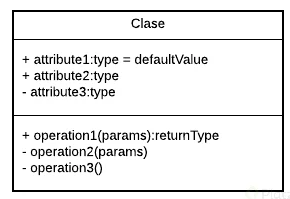
\includegraphics[scale=0.5]{2.1.png}\\
En la parte superior se colocan los atributos o propiedades, y debajo las operaciones de la clase. Notarás que el primer caracter con el que empiezan es un símbolo. Este denotará la visibilidad del atributo o método, esto es un término que tiene que ver con Encapsulamiento y veremos más adelante a detalle.\\
Estos son los niveles de visibilidad que puedes tener:
\begin{enumerate}
    \item $-$  private
    \item $+$  public
    \item $\#$  protected
    \item $~$  default
\end{enumerate}

Una forma de representar las relaciones que tendrá un elemento con otro es a través de las flechas en UML, y aquí tenemos varios tipos, estos son los más comunes:
\subsubsection*{Asociación}
Como su nombre lo dice, notarás que cada vez que esté referenciada este tipo de flecha significará que ese elemento contiene al otro en su definición.\\
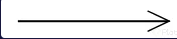
\includegraphics[scale=0.5]{2.2.png}\\
La flecha apuntará hacia la dependencia.\\
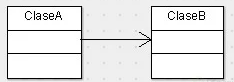
\includegraphics[scale=0.5]{2.3.png}\\
Con esto vemos que la ClaseA está asociada y depende de la ClaseB.
\subsubsection*{Herencia}
Siempre que veamos este tipo de flecha se estará expresando la herencia.\\
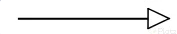
\includegraphics[scale=0.5]{2.4.png}\\
La dirección de la flecha irá desde el hijo hasta el padre.\\
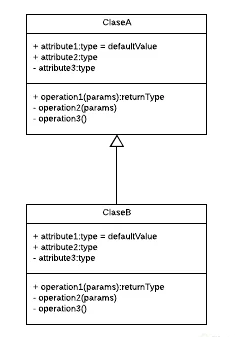
\includegraphics[scale=0.5]{2.5.png}\\
Con esto vemos que la ClaseB hereda de la ClaseA
\subsubsection*{Agregación}
Este se parece a la asociación en que un elemento dependerá del otro, pero en este caso será: Un elemento dependerá de muchos otros.\\

\includegraphics[scale=0.5]{2.6.png}\\
Aquí tomamos como referencia la multiplicidad del elemento. Lo que comúnmente conocerías en Bases de Datos como Relaciones uno a muchos.\\
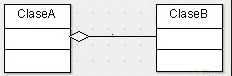
\includegraphics[scale=0.5]{2.7.png}\\
Con esto decimos que la ClaseA contiene varios elementos de la ClaseB. Estos últimos son comúnmente representados con listas o colecciones de datos.
\subsubsection*{Composición}
Este es similar al anterior solo que su relación es totalmente compenetrada.\\

\includegraphics[scale=0.5]{2.8.png}\\
De tal modo que conceptualmente una de estas clases no podría vivir si no existiera la otra.\\
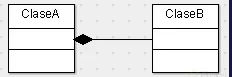
\includegraphics[scale=0.5]{2.9.png}\\

\newpage
\section{JAVA orientada a objetos}
Java es un lenguaje de programación orientado a objetos (POO) que se ha convertido en uno de los más populares en la actualidad. Su éxito se debe en gran medida a su capacidad para manejar de manera eficiente la programación orientada a objetos. 
\subsection{Clase}
\begin{lstlisting}
class Person{
    String name = "";
    void walk(){

    }
} 
\end{lstlisting}
Este fregmento define una clase llamada "Person" que tiene un atributo "name" de tipo String y un método "walk" que no hace nada.

\subsection{Ejemplo práctico: Sistema de gestión de una biblioteca}

Imaginemos que queremos crear un sistema de gestión de una biblioteca en Java. Para ello, podemos utilizar los conceptos de modularidad, abstracción, polimorfismo, herencia y encapsulamiento.

\subsubsection*{Modularidad}

La modularidad se refiere a la división del código en módulos independientes que pueden ser desarrollados, probados y mantenidos por separado. En nuestro sistema de gestión de biblioteca, podemos utilizar la modularidad para dividir el código en diferentes clases, cada una de las cuales es responsable de una funcionalidad específica. Por ejemplo, podemos tener una clase para la gestión de libros, otra clase para la gestión de usuarios, y otra clase para la gestión de préstamos.

\subsubsection*{Abstracción}

La abstracción se refiere a la capacidad de ocultar los detalles complejos y mostrar sólo la información esencial. En nuestro sistema de gestión de biblioteca, podemos utilizar la abstracción para crear una clase abstracta llamada \texttt{Item} que representa tanto a los libros como a otros elementos de la biblioteca, como DVDs o CDs. Esta clase podría contener métodos y propiedades que son comunes a todos los elementos de la biblioteca, como un número de identificación y un título.

\subsubsection*{Polimorfismo}

El polimorfismo se refiere a la capacidad de los objetos de tomar diferentes formas. En nuestro sistema de gestión de biblioteca, podemos utilizar el polimorfismo para crear diferentes tipos de elementos de la biblioteca, como libros y DVDs, que heredan de la clase \texttt{Item} y tienen sus propios métodos y propiedades únicas. Podríamos tener una clase \texttt{Book} que hereda de la clase \texttt{Item} y tiene propiedades como el autor y la fecha de publicación, y una clase \texttt{DVD} que también hereda de \texttt{Item} y tiene propiedades como la duración y el género.

\subsubsection*{Herencia}

La herencia se refiere a la capacidad de las clases hijas de heredar propiedades y métodos de la clase padre. En nuestro sistema de gestión de biblioteca, podemos utilizar la herencia para crear una jerarquía de clases en la que las clases hijas heredan propiedades y métodos de la clase padre. Por ejemplo, la clase \texttt{Book} podría heredar de la clase \texttt{Item} y tener acceso a sus propiedades y métodos.

\subsubsection*{Encapsulamiento}

El encapsulamiento se refiere a la capacidad de ocultar los detalles de implementación y proteger los datos y métodos de una clase de acceso no autorizado. En nuestro sistema de gestión de biblioteca, podemos utilizar el encapsulamiento para proteger los datos de los elementos de la biblioteca y limitar el acceso a ellos. Podemos definir las propiedades y métodos de la clase \texttt{Item} como privados para que sólo puedan ser accedidos y modificados por métodos dentro de la misma clase.

Para el ejemplo Es útil realizar el diagrama UML:\\
\begin{center}
    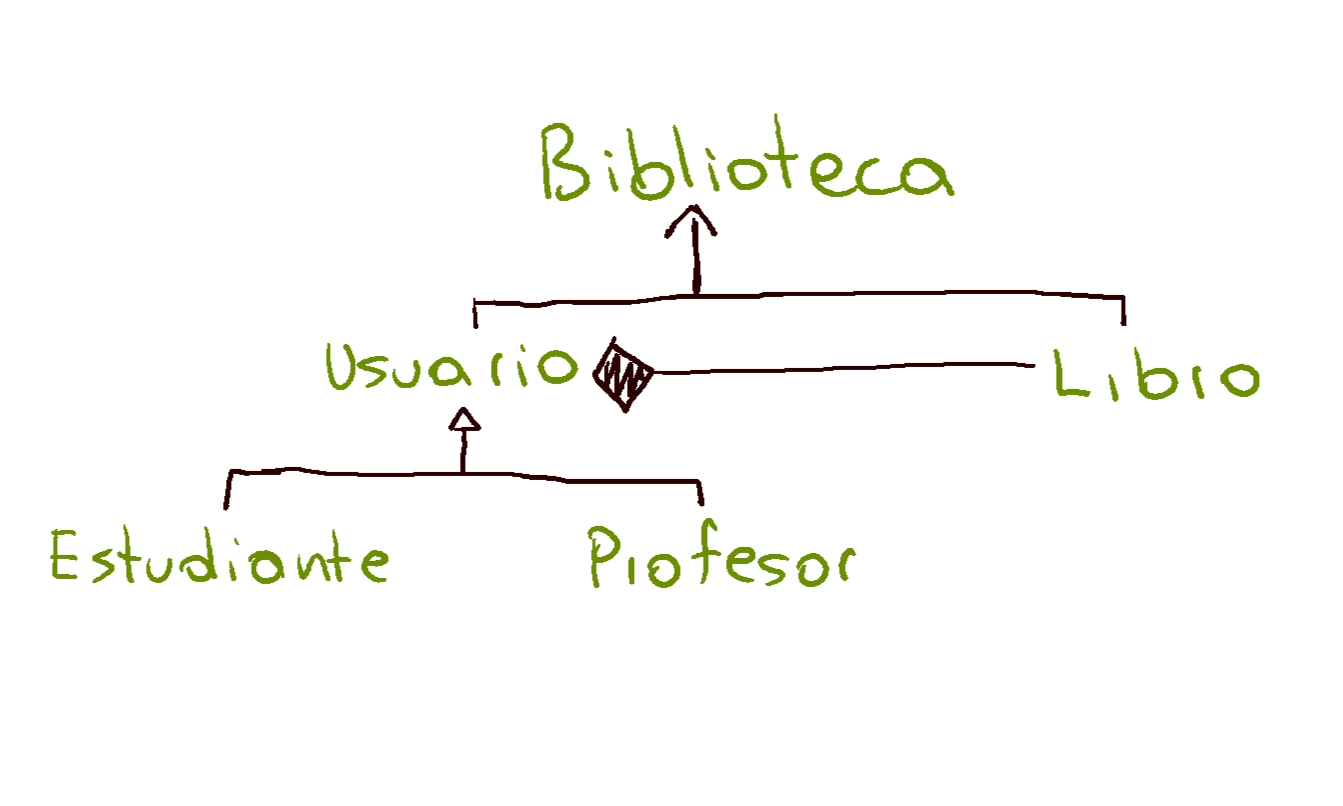
\includegraphics[scale=0.2]{3.1.png}\\ 
\end{center}
Donde\\
\begin{center}
    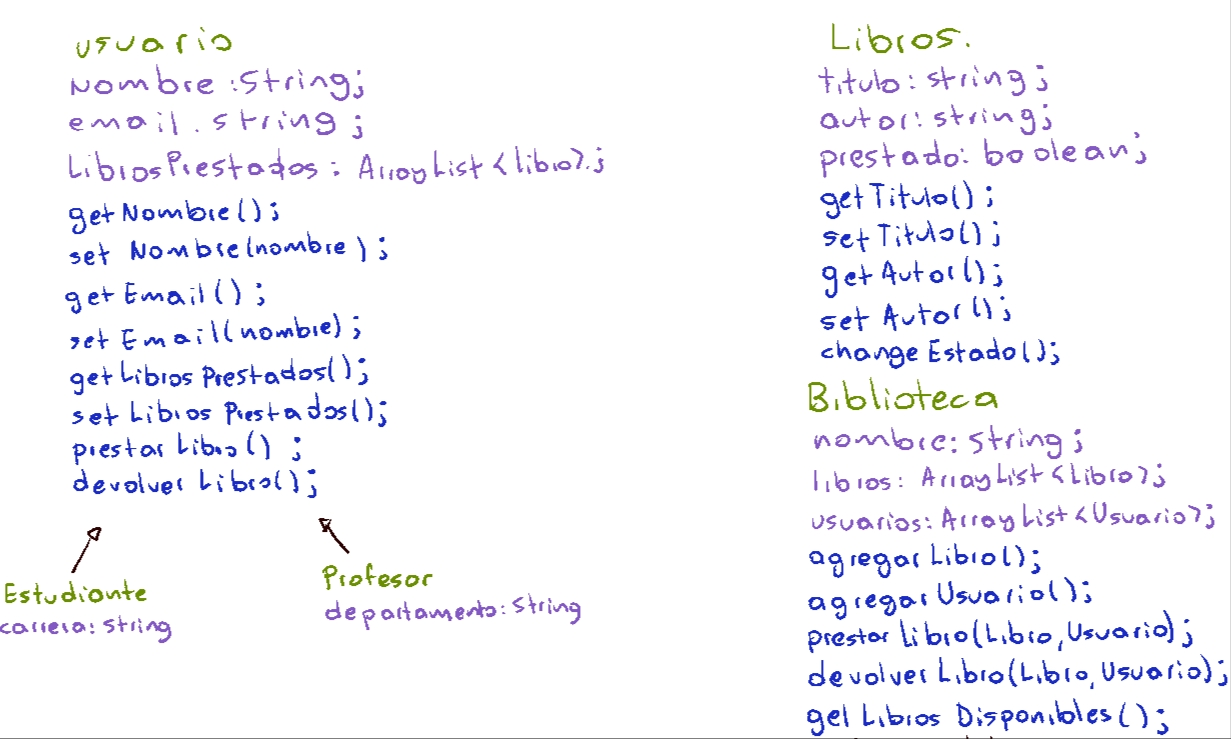
\includegraphics[scale=0.3]{3.2.png}\\ 
\end{center}

Comencemos a escribir codigo:\\ 
Creamos la clase Biblioteca:
\begin{lstlisting}
import java.lang.reflect.Array;
import java.util.ArrayList;

public class Biblioteca {
    private String nombre;
    private ArrayList<Libro> libros;
    private ArrayList<Usuario> usuarios;

    public Biblioteca(String nombre) {
        this.nombre = nombre;
        libros = new ArrayList<Libro>();
        usuarios = new ArrayList<Usuario>();
    }

    public void agregarLibro(Libro libro) {
        libros.add(libro);
    }

    public void agregarUsuario(Usuario usuario) {
        usuarios.add(usuario);
    }

    public void prestarLibro(Libro libro, Usuario usuario) {
        if (libros.contains(libro) && !libro.prestado) {
            libro.changeEstado();
            usuario.prestarLibro(libro);
            System.out.println("El libro " + libro.getTitulo() + " ha sido prestado a " + usuario.getNombre());
        } else {
            System.out.println("No se puede prestar el libro " + libro.getTitulo() + " a " + usuario.getNombre());
        }
    }

    public void devolverLibro(Libro libro, Usuario usuario) {
        if (libros.contains(libro) && !libro.prestado) {
            usuario.devolverLibro(libro);
            usuario.devolverLibro(libro);
            libro.changeEstado();
            System.out.println("El libro " + libro.getTitulo() + " ha sido devuelto por " + usuario.getNombre());
        }
    }
    public ArrayList<Libro> getLibrosDisponibles() {
        ArrayList<Libro> librosDisponibles = new ArrayList<Libro>();
        for(Libro libro : libros){
            if(!libro.prestado){
                librosDisponibles.add(libro);
                System.out.println("El libro " + libro.getTitulo() + " Esta disponible");
            }
        }
        return librosDisponibles;
    }
}
\end{lstlisting}
Y hablando de herencia, podemos podemos agregar una clase Usuario y luego crear dos subclases Estudiante y Profesor que hereden de ella. De esta manera, los objetos de tipo Estudiante y Profesor tendrán todos los atributos y métodos de la clase Usuario, además de los propios.
\begin{lstlisting}
import java.util.ArrayList;

class Usuario {
    private String nombre;
    private String email;
    private ArrayList<Libro>librosPrestados;
    public Usuario(String nombre, String email) {
        this.nombre = nombre;
        this.email = email;
        this.librosPrestados = new ArrayList<Libro>();
    }

    public String getNombre() {
        return nombre;
    }

    public void setNombre(String nombre) {
        this.nombre = nombre;
    }

    public String getEmail() {
        return email;
    }

    public void setEmail(String email) {
        this.email = email;
    }

    public ArrayList<Libro> getLibrosPrestados() {
        return librosPrestados;
    }

    public void setLibrosPrestados(ArrayList<Libro> librosPrestados) {
        this.librosPrestados = librosPrestados;
    }

    public void prestarLibro(Libro libro) {
        librosPrestados.add(libro);
    }

    public void devolverLibro(Libro libro) {
        librosPrestados.remove(libro);
    }

    @Override
    public String toString() {
        return "Usuario [nombre=" + nombre + ", email=" + email + ", librosPrestados=" + librosPrestados + "]";
    }
}

class Estudiante extends Usuario {
    private String carrera;

    public Estudiante(String nombre, String email, String carrera) {
        super(nombre,email);
        this.carrera = carrera;
    }

    public String getCarrera() {
        return carrera;
    }
}

class Profesor extends Usuario {
    private String departamento;

    public Profesor(String nombre, String email, String carrera) {
        super(nombre,email);
        this.departamento = departamento;
    }

    public String getDepartamento() {
        return departamento;
    }
}
\end{lstlisting}
Aquí hemos creado dos subclases Estudiante y Profesor que heredan de la clase Usuario. Ahora podemos crear objetos de estas subclases y usar todos los métodos y atributos de la clase Usuario, además de los métodos y atributos adicionales de cada subclase. Por ejemplo, podemos crear un objeto Estudiante.

Pero también debemos crear la clase Libro:
\begin{lstlisting}
class Libro {
    private String titulo;
    private String autor;
    public boolean prestado;

    public Libro(String titulo, String autor) {
        this.titulo = titulo;
        this.autor = autor;
        this.prestado = false;
    }
    public void changeEstado() {
        this.prestado = !prestado;
    }
    public String getTitulo() {
        return titulo;
    }

    @Override
    public String toString() {
        return "Libro [titulo=" + titulo + ", autor=" + autor +  ", prestado="
                + prestado + "]";
    }
}
\end{lstlisting}

Mostremos un ejemplo de cómo se podría instanciar y usar los métodos de las clases que hemos definido:
\begin{lstlisting}
public class Main {
    public static void main(String[] args) {
        Biblioteca biblioteca = new Biblioteca("Biblioteca Municipal");

        // Agregamos algunos libros a la biblioteca
        Libro libro1 = new Libro("100 a~nos de soledad", "Gabriel Garc'ia M'arquez");
        Libro libro2 = new Libro("El Aleph", "Jorge Luis Borges");
        Libro libro3 = new Libro("Rayuela", "Julio Cort'azar");
        biblioteca.agregarLibro(libro1);
        biblioteca.agregarLibro(libro2);
        biblioteca.agregarLibro(libro3);

        // Agregamos algunos usuarios a la biblioteca
        Usuario usuario1 = new Usuario("Juan", "P'erez");
        Usuario usuario2 = new Usuario("Mar'ia", "Gonz'alez");
        biblioteca.agregarUsuario(usuario1);
        biblioteca.agregarUsuario(usuario2);

        // Imprimimos la informaci'on del libro 1
        System.out.println(libro1);

        // Imprimimos los libros que est'an disponibles en la biblioteca
        System.out.println("Libros disponibles:");
        biblioteca.getLibrosDisponibles();
    }
\end{lstlisting}
Cuando lo ejecutemos la salida será:
\begin{verbatim}
Libro [titulo=100 años de soledad, autor=Gabriel García Márquez, prestado=false]
Libros disponibles:
El libro 100 años de soledad Está disponible
El libro El Aleph Está disponible
El libro Rayuela Está disponible

Process finished with exit code 0
\end{verbatim}

\newpage
\section{Bibliografía}
\begin{thebibliography}{9}
\bibitem{clean-code} Martin, Robert C. \textit{Clean Code: A Handbook of Agile Software Craftsmanship}. Prentice Hall, 2008.
\bibitem{platzi-java-basico} Platzi. \textit{Curso de Java Básico}. Platzi, 2023.\\ \url{https://platzi.com/cursos/java-basico/}
\bibitem{platzi-java-oo} Platzi. \textit{Curso de Java Orientado a Objetos}. Platzi, 2023.\\ \url{https://platzi.com/cursos/java-poo/}
\bibitem{java-docs} Oracle Corporation. \textit{Java SE Documentation}. Oracle Corporation, 2023.\\ \url{https://docs.oracle.com/en/java/javase/index.html}
\end{thebibliography}



\end{document}